\documentclass[border=4pt,varwidth=17cm]{standalone}
\usepackage{amsmath,amssymb,mathrsfs,mathtools}
\usepackage{tikz}
\usetikzlibrary{positioning,fit,backgrounds,arrows.meta}
\def\RR{{\mathbb R}}\def\eps{\varepsilon}\def\then{\Rightarrow}
\def\J{\mathcal{J}_L}\def\A{\mathcal{A}_{f,g}}\def\Sol{\mathcal{S}_{f,g}}
\def\limsup{\mathop{\overline{\lim}}}\def\liminf{\mathop{\underline{\lim}}}
\def\Of{{\sf (O$_f$)}}\def\Og{{\sf (O$_g$)}}
\def\Rv{{\sf (R$_{\rm v}$)}}\def\Rh{{\sf (R$_{\rm h}$)}}
\begin{document}


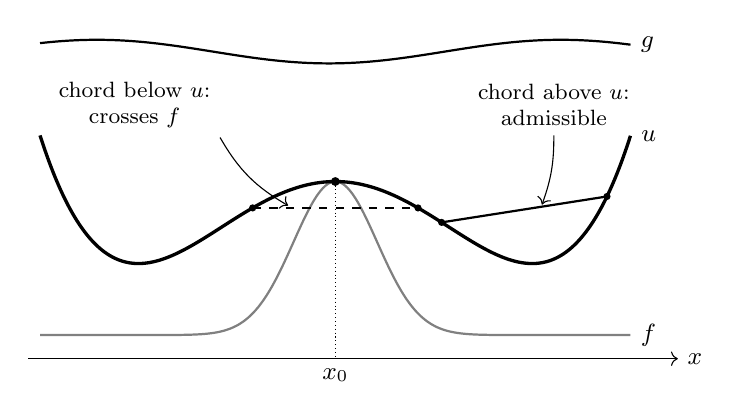
\begin{tikzpicture}[x=1.5cm, y=1.5cm, font=\small,
  declare function={U(\t)=1.5-0.5*(\t-3)^2+0.09*(\t-3)^4; F(\t)=0.2+1.3*exp(-(\t-3)^2/0.25);}]
  % obstacles and solution
  \draw[thick, domain=0.5:5.5, samples=60, smooth] plot (\x, {2.6+0.1*sin(deg(1.6*\x))}) node[right] {$g$};
  \draw[thick, gray, domain=0.5:5.5, samples=120, smooth] plot (\x, {F(\x)}) node[right, black] {$f$};
  \draw[very thick, domain=0.5:5.5, samples=120, smooth] plot (\x, {U(\x)}) node[right] {$u$};
  % contact point
  \fill (3,1.5) circle (1.6pt);
  \draw[densely dotted] (3,1.5) -- (3,0) node[below] {$x_0$};
  % chord below u: crosses f
  \draw[thick, dashed] (2.3,{U(2.3)}) -- (3.7,{U(3.7)});
  \fill (2.3,{U(2.3)}) circle (1.3pt) (3.7,{U(3.7)}) circle (1.3pt);
  \node[align=center, font=\footnotesize] (nb) at (1.3,2.15) {chord below $u$:\\ crosses $f$};
  \draw[->, thin] (nb.south east) to[bend right=15] (2.6,{U(2.3)+0.02});
  % chord above u: admissible
  \draw[thick] (3.9,{U(3.9)}) -- (5.3,{U(5.3)});
  \fill (3.9,{U(3.9)}) circle (1.3pt) (5.3,{U(5.3)}) circle (1.3pt);
  \node[align=center, font=\footnotesize] (na) at (4.85,2.15) {chord above $u$:\\ admissible};
  \draw[->, thin] (na.south) to[bend left=10] (4.75,{(U(3.9)*0.45+U(5.3)*0.55)+0.03});
  % axis
  \draw[->] (0.4,0) -- (5.9,0) node[right] {$x$};
\end{tikzpicture}


\end{document}
